\chapter{Proportional EMG-Driven Angle Control}
\label{ch:ProportionalControl}

Many authors applied successfully a proportional EMG control for a mechanism (e.g. \cite{Bottomley411}). Hogan \cite{1103644} stated that, for contractions of the muscle below 30\% of the maximum voluntary contraction, the relative force applied by the biceps muscle to the elbow joint and the EMG signal can be considered as proportional. 

Lets assume a simplified model of the arm with one degree of freedom on the elbow joint. 

\begin{equation}\label{eq:simpleModel}
T = (J + M\cdot L^2)\cdot \ddot{\theta}  + B \cdot \dot{\theta}  + (m\cdot l + M \cdot L) \cdot g \cdot cos(\theta)
\end{equation}


If we assume low speed and low acceleration, the equation can be simplified to:

\begin{equation}\label{eq:kcos}
T = K \cdot cos(\theta)
\end{equation}

\begin{equation}
K = (m\cdot l + M\cdot L)\cdot g
\end{equation}

Where K is the coefficient for the gravity-related forces.

This equation states a direct relationship between joint angle and torque and consequently, for low muscle activation levels, joint angle and EMG magnitude.

From the experiments developed at chapter \ref{ch:preliminarExperiment}, a powerful relation between the elbow angle and the sEMG signal can be observed, especially at the test set where the user is carrying no extra weight in his hand, shown in figure \ref{EmgAngleDirect}.

\begin{figure}[thpb]
      \centering
      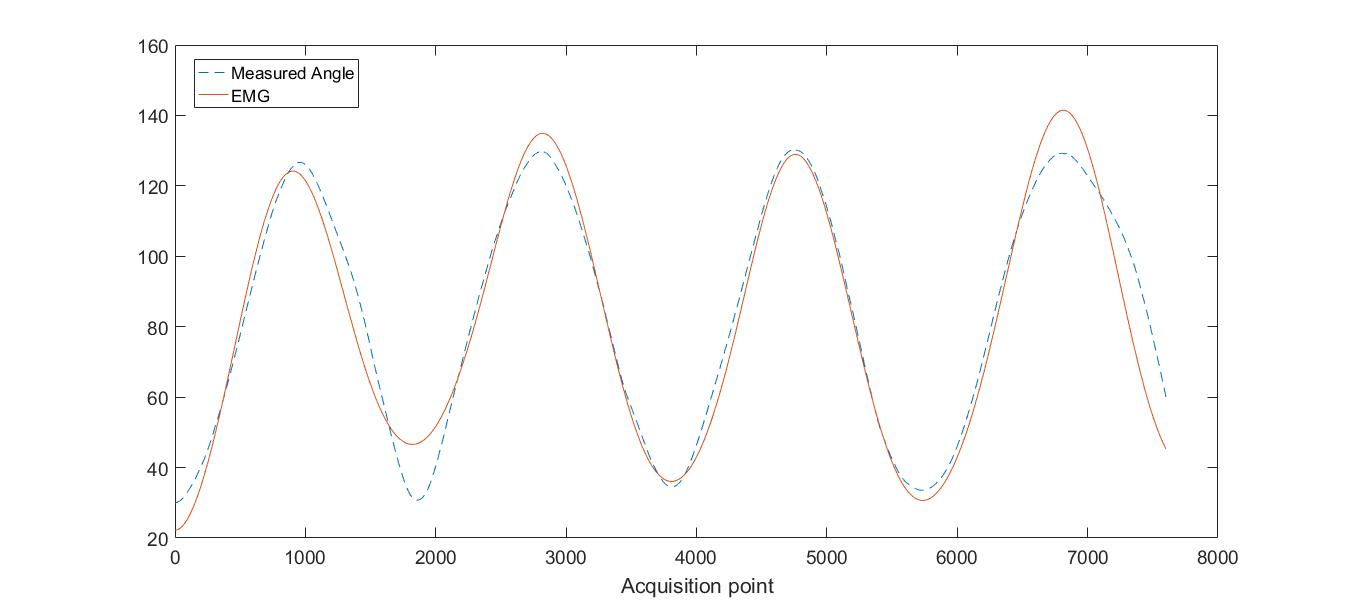
\includegraphics[scale=0.35]{Images/EmgAngleDirect.jpg}
      \caption{Comparison between the measured elbow angle and the EMG values for the continuous movement. The EMG values were multiplied by a constant for better visualization.}
      \label{EmgAngleDirect}
   \end{figure}
   
   The correlation between these two signals is 97.78\%. It shows that, at least for the configuration of the proposed experiment, there is a high correlation between the EMG signal and the elbow joint angle.
   
   The first problem of this relation appears when comparing the EMG signals with the intermittent movement. See figure \ref{EmgAngleInt}.

\begin{figure}[thpb]
      \centering
      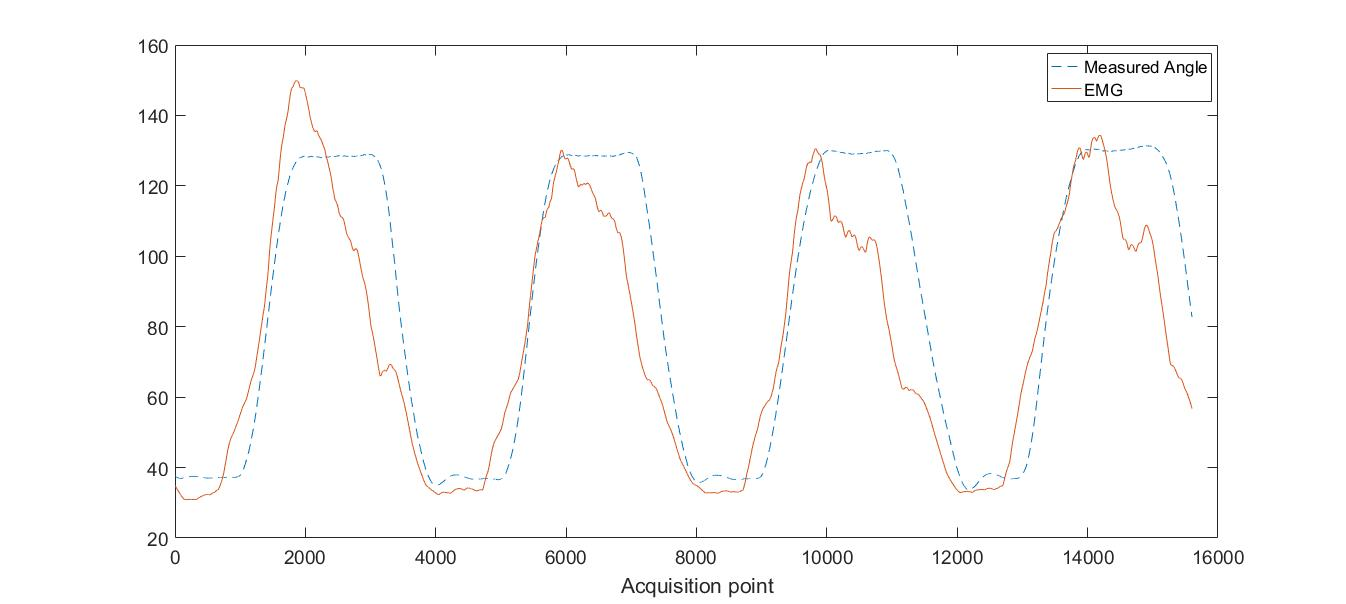
\includegraphics[scale=0.35]{Images/EmgAngleInt.jpg}
      \caption{Comparison between the measured elbow angle and the EMG values for the intermittent movement. The EMG values were multiplied by a constant for better visualization.}
      \label{EmgAngleInt}
   \end{figure}
   
   As the image shows, for the upward movement, there is a proportional relation between the EMG values and the angle of the elbow joint. When the elbow joint stays in a static angle, the EMG magnitude lowers, even without elbow movement. 
   
   
   To address this problem, further investigations must be made. Two main ideias will be explored. The first one is to use the Time Domain analysis of the EMG signal. The TD analysis is commonly used in pattern recognition for EMG signals. It uses the Mean Absolute Value,
Zero Crossing, Slope Sign Changes and Waveform Length of the signal to acquire more information about the user's intention of movement. Another ideia is to use the wavelet analysis to the EMG signal. The wavelet analysis is extensively used in EMG pattern recognition systems. It analyses a larger bandwidth than just the 1Hz to 3Hz commonly used in EMG proportional control. By analyzing higher frequencies, it is possible to acquire more information about the intention of movement. "Borrowing" this technique to the proportional control, we may be able to detect the intention to make an extension movement and then using the proportional control to determine the desired position of the joint.